\section{Local Area Networks}
Local area networks, generally called LANs, are privately-owned 
networks within a single building or campus of 
up to a few kilometers in size. LANs are 
distinguished from other kinds of networks by three  
characteristics:
  
\begin{itemize}
  \item their size, 
  \item their transmission technology, and
  \item their topology.  
\end{itemize}

LANs are restricted in size,  which means that the 
worst-case transmission time is bounded and known in 
advance. Knowing this bound makes it possible to use 
certain kinds of designs that would not otherwise 
be possible. It also simplifies network management. 
LANs may use a transmission technology consisting 
of a ¿¿¿¿¿¿¿cable??????? to which all the machines 
are attached. Traditional  LANs  run  at  
speeds  of  10  Mbps  to  100 
Mbps, have low delay (microseconds or nanoseconds), 
and make very few errors. Newer LANs operate at up to 
10 Gbps. 

Various topologies are possible for broadcast LANs. 
Figure \ref{fig:lan-networks-topologies-fig} shows 
two of them. In a 
bus (i.e., a linear cable) network, 
at any instant at most one machine is the master 
and is allowed to transmit. All other machines are 
required to refrain from sending. An arbitration 
mechanism is needed to resolve conflicts when two or more 
machines want to transmit simultaneously. The 
arbitration mechanism may be centralized or 
distributed. IEEE 802.3, popularly called Ethernet, 
for example, is a bus-based broadcast network with 
decentralized control, usually operating at 10 Mbps 
to 10 Gbps. Computers on an Ethernet can transmit 
whenever they want to; if two or more packets collide, 
each computer just waits a random time and tries again later. 


\begin{figure}
  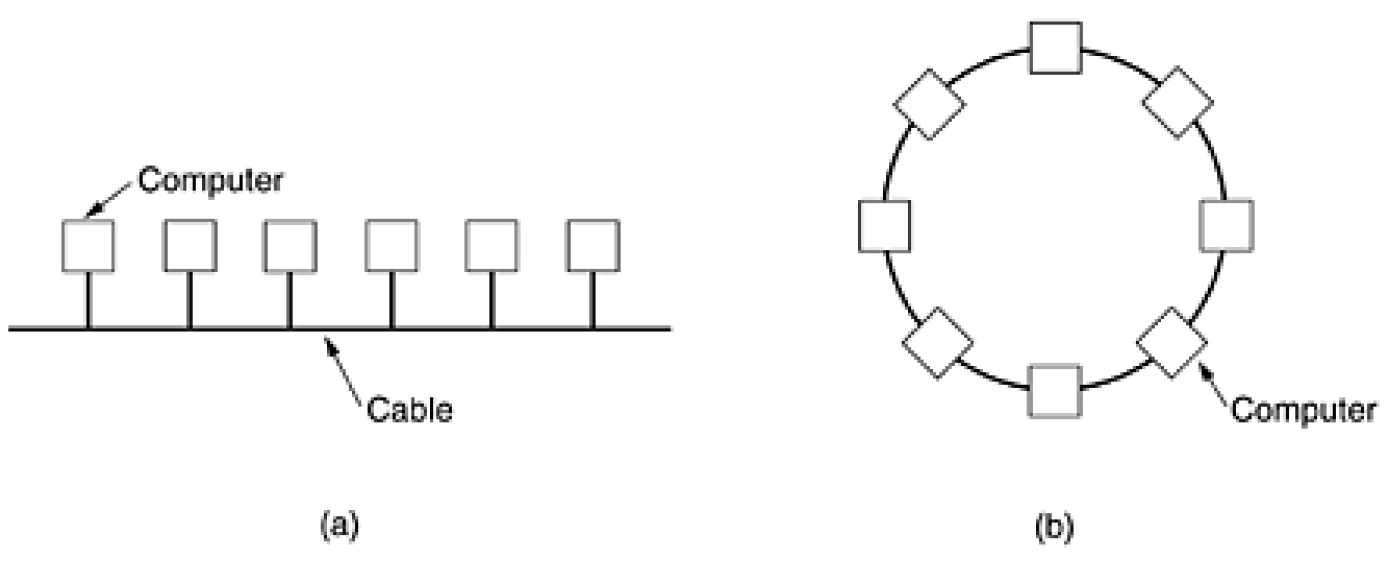
\includegraphics[width=1.0\textwidth]{chapters/ch-networks/figures/lan-networks-topologies}
  \caption{Two broadcast networks. (a) Bus. (b) Ring \cite{Tanembaum:2003cn}}
  \label{fig:lan-networks-topologies-fig}
\end{figure}